\section{Git}
\label{sec:git}
  Git is a very useful tool in teamwork development. All our members used it for a long time so we use it well.
  Merge, rebase and commits show our professional develop skill and the great work we had done.
  \begin{figure}[H]
    \centering
    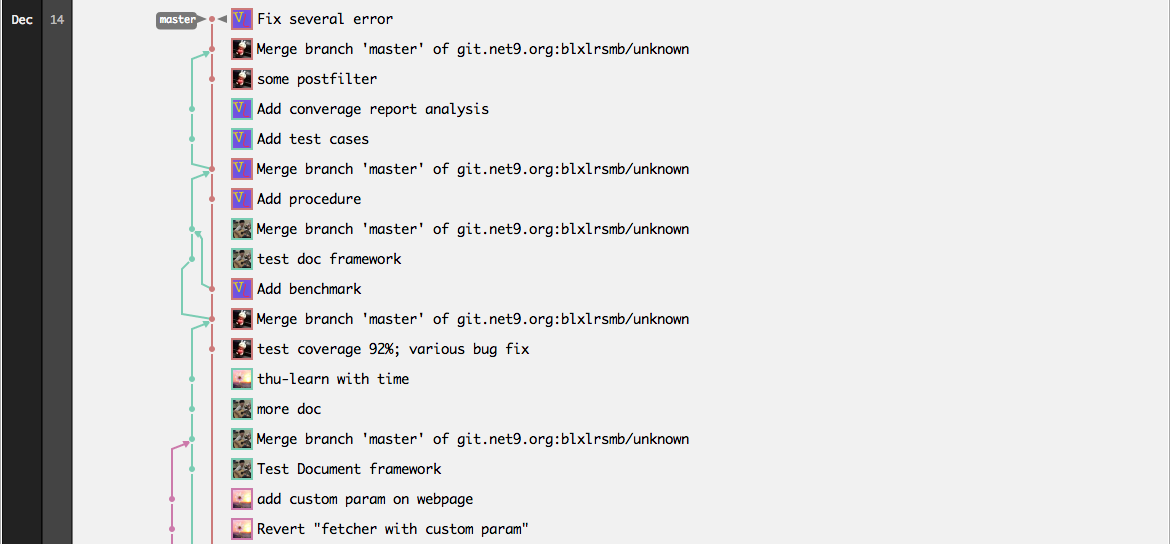
\includegraphics[width=0.8\textwidth]{img/commits.png}
    \caption{Recent Commits\label{fig:commits}}
  \end{figure}
  \begin{figure}[H]
    \centering
    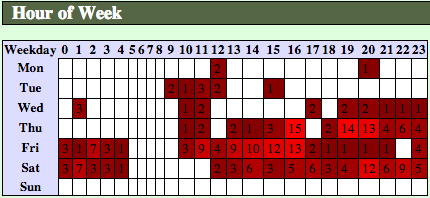
\includegraphics[width=0.8\textwidth]{img/workhour.png}
    \caption{Work Hours\label{fig:workhour}}
  \end{figure}
  \begin{figure}[H]
    \centering
    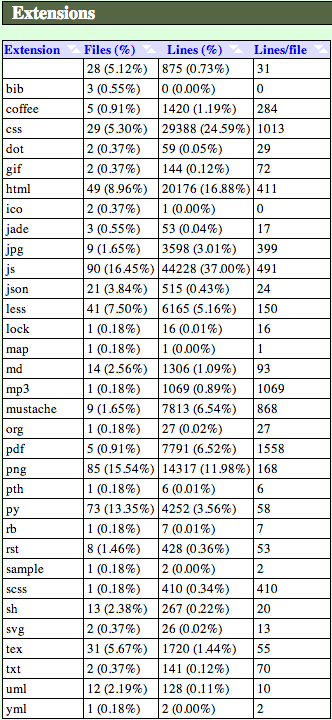
\includegraphics[width=0.5\textwidth]{img/files.png}
    \caption{Tracked Files\label{fig:files}}
  \end{figure}
\section{Issues}
\label{sec:issue}
  Issue Tracker is very common used in develop management. It can record the progress of a feature, a fix procedure of a bug, and so on.
  Every issue as a assignee that has responsibility for that issue with a deadline. Discussions can also be made and recorded under that.

  Up to now, we had created 33 issues, resolved 31 of them, most of which are features.
  \begin{figure}[H]
    \centering
    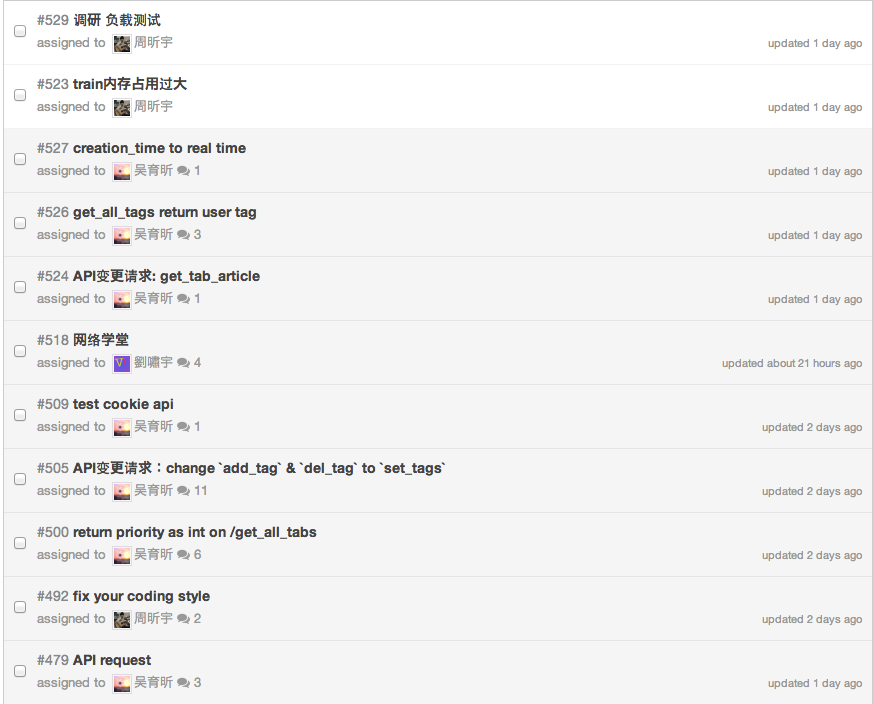
\includegraphics[width=\textwidth]{img/issue.png}
    \caption{Parts of Issues\label{fig:issue}}
  \end{figure}

  The issues are listed below:
  \begin{description}
    \item[Using Python3 instead of Python2]{Unify the develop language version}
    \item[Fetcher的架构设计]{Design of system}
    \item[Fetcher prototype implement]{Prototype system demo}
    \item[about de requirement doc]{Document draft writing}
    \item[求一个logo!]{Design a fantasy logo}
    \item[Add UML]{Document enhancement}
    \item[给这个图加几条线]{Document enhancement}
    \item[设计文档]{Document draft writing}
    \item[Fix PEP8]{Coding style problem}
    \item[OAuth with OAuth]{Feature (wont fix)}
    \item[门户网站信息获取]{Feature}
    \item[客户端网站界面设计]{Design feature}
    \item[apiwebsite简单实现]{Demo}
    \item[初级分类器prefilter简单实现]{Demo}
    \item[多写一些例子]{Cooperation problem}
    \item[注册实现]{Feature}
    \item[登路 登出实现]{Feature}
    \item[前端框架搭建]{Feature}
    \item[求在一台服务器上跑起来能用API]{Deploy}
    \item[API request]{Feature}
    \item[fix your coding style]{Coding style problem}
    \item[return priority as int on /get\_all\_tabs]{Feature}
    \item[API变更请求:change `add\_tag' \& `del\_tag' to `set\_tags']{Feature}
    \item[test cookie api]{Feature}
    \item[网络学堂]{Feature}
    \item[train内存占用过大]{System enhancement}
    \item[API变更请求: get\_tab\_article]{Feature}
    \item[get\_all\_tags return user tag]{Feature}
    \item[creation\_time to real time]{System enhancement}
    \item[调研 负载测试]{Test}
    \item[前端bug]{Bug}
    \item[前10条]{System enhancement}
    \item[展示用ppt]{Presentation}
  \end{description}
